\newif\ifcommentenabled \commentenabledtrue
\newcommand{\TS}[1]{\ifcommentenabled\textcolor{red}{TS: #1}\fi}

\documentclass[12pt, a4paper, titlepage]{report}
\usepackage[dvipdfmx]{graphicx}
\usepackage[nottoc,numbib]{tocbibind}
\usepackage[utf8]{inputenc}
\usepackage{amsmath}
\usepackage{color}
\usepackage{enumerate}
\usepackage{hyperref}
\usepackage{mathptmx}
\usepackage{minted}
\usepackage{pdfpages} % PDF inclusion
\usepackage{verbatim} % comment environment
\hypersetup{
  colorlinks = true,
  linkcolor = cyan
}

% Title Page
\title{Bachelor Thesis \\ TODO: TITLE}
\author{
  03190413 Takemaru Kadoi
  \\[1cm]
  {\small Supervisor: Prof. Masahiro Fujita},
  {\small Advisor: Assistant Prof. Taro Sekiyama}
  \\[1cm]
  {\small University of Tokyo, Department of Information and Communication Engineering}
}
\date{\today}

\begin{document}

% front page
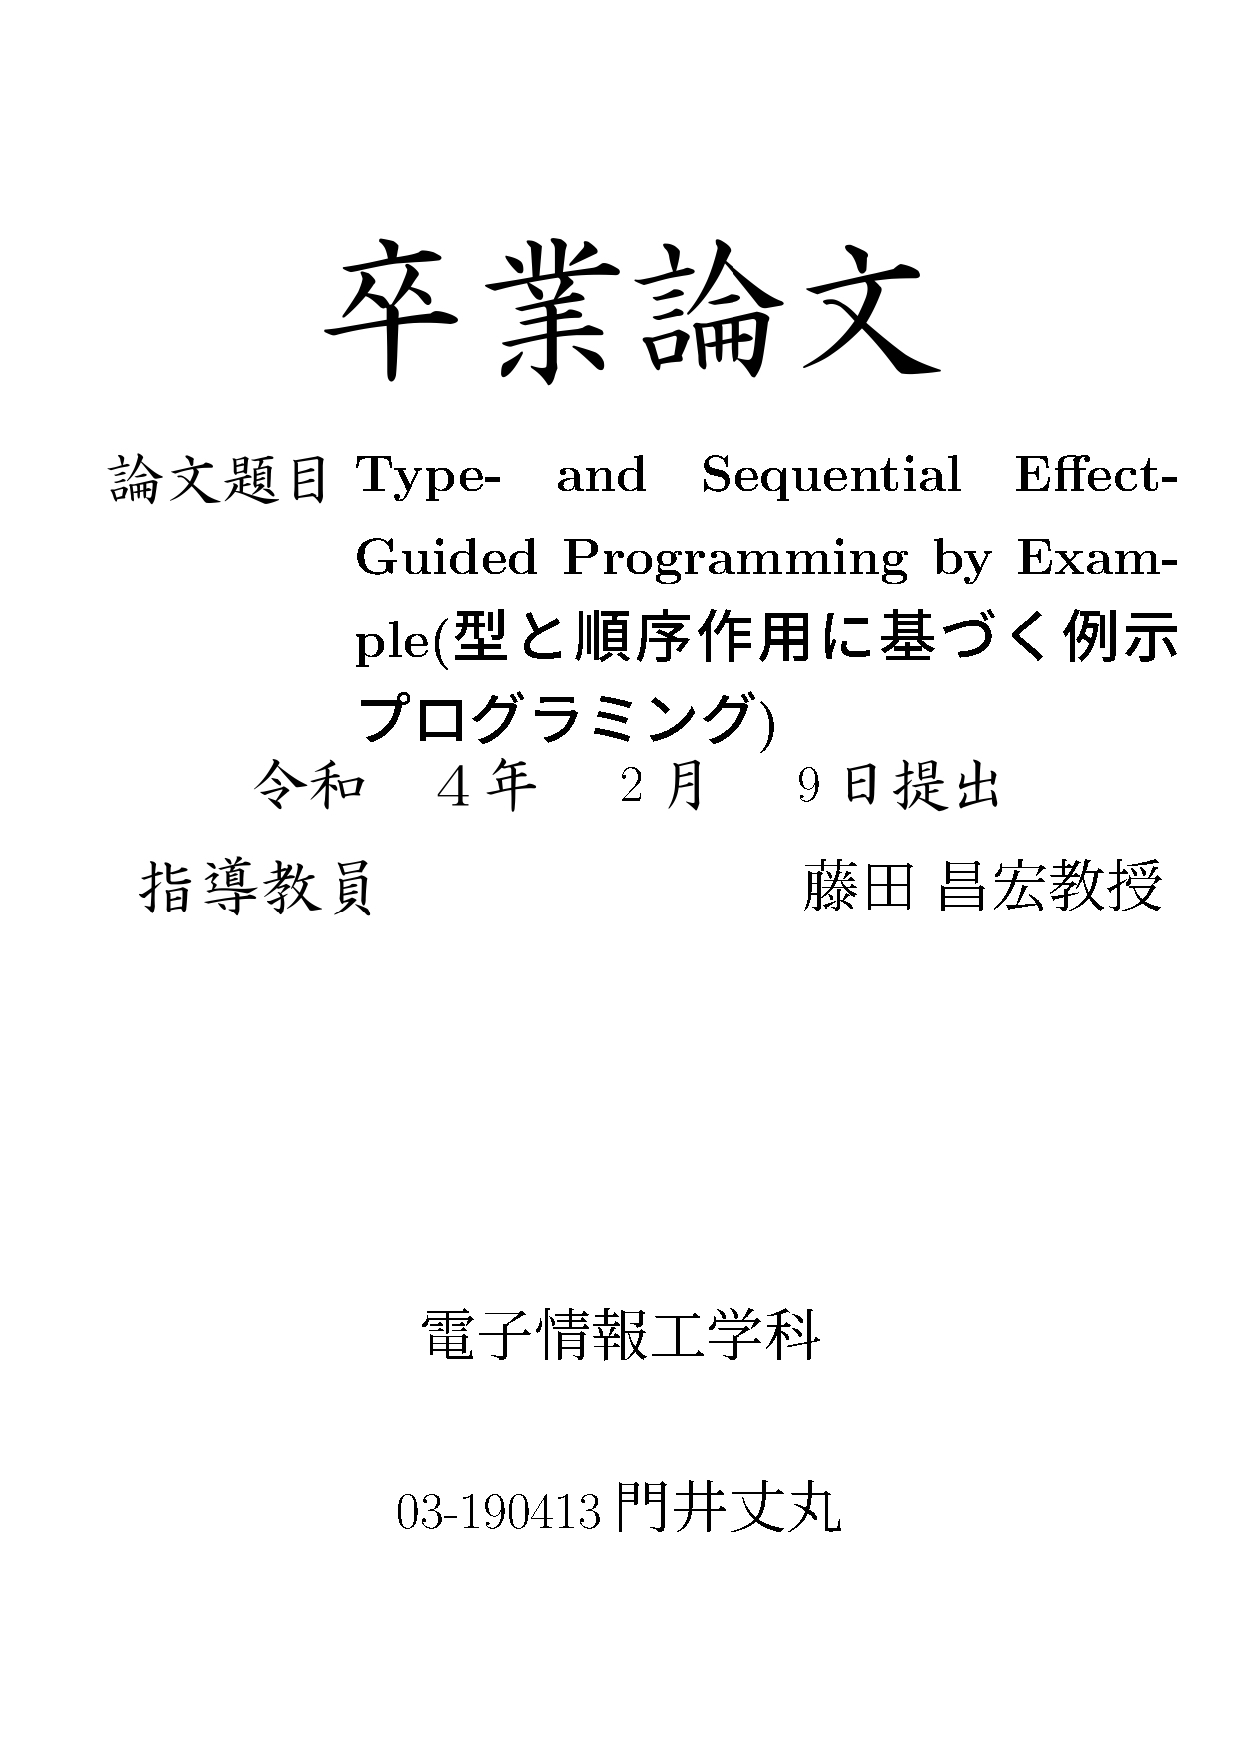
\includepdf[pages={-}]{images/sotsuronFront.pdf}

% header
\maketitle
\newpage
\tableofcontents
\newpage

\chapter*{Acknowledgment}
This research was supervised by Prof. Fujita at the University of Tokyo and supported by Assistant Prof. Sekiyama at National Institute of Technology. \\
I thank my colleagues at the University of Tokyo, Miyasaka-san, Koike-san, Yu-san, Nagasawa-san, and Yi-san.
% TODO: add twitter accounts
I also show my gratitude to my good friends, hnkz, Akio, Saeki, Arahata, Hori, Naito, Chen, and Sakura.

% overview of the research topic
\chapter{Abstract} \label{section:abstract}
In recent years, several tools have been developed to enhance the productivity of programmers.
In particular, tools for generating code have attracted a lot of attention, and program synthesis is a research field that supports this development.
Program synthesis requires specifications with which users tell a computer what they want to achieve.
In the case of logical formulae \TS{expressions $\rightarrow$ formulas / formulae} , it is
difficult for programmers who are not skilled in math while its strictness contributes to accurate code generation. \TS{The advantages of logical formulas should be described.}
With natural language, computers may not be able to understand the meaning, and the intention may not be conveyed correctly even though programmers can find it easy to write specifications. \TS{What are the advantages of specifications in natural languages?}
This paper examines the use of a type and effect system as a specification that is easy to understand by \TS{both} humans and computers alike. The types are properties of data and can be used to describe the input and output of a function. The effects, which can explain the internal processes of a function, represent a transition in a state, such as the value of a variable, shared memory between threads, and I/O operations.
\TS{What are types and effects?}
Types are familiar to programmers who use statically typed languages.
Many users are unfamiliar with effects, but the effects \TS{What "they" means is a bit ambiguous. It is clearer to say "effects".} can describe the internal behavior of programs \TS{Here is the first place you mention functions, so it sounds abrupt.  It may be natural to say "code" or "programs"} and are easy to understand if designed properly.
By utilizing type and effect, I can efficiently explore candidate code and demonstrate that the intended code will be generated. I will demonstrate some specifications and an example of a program that has been generated based on these specifications.
\TS{How do you synthesize programs with types and effects?  What experiments are (planed to be) conducted?  How about results?}

In Chapter \ref{section:introduction}, I discuss the motivation for this research, what program synthesis is, and existing methods.
I explain my proposed method in Chapter \ref{section:method}.
I present in Chapter \ref{section:experiment} the results obtained by the proposed method and evaluate them.
Chapter \ref{section:conclusion} concludes with a summary of the results and evaluation, as well as future issues.

\chapter{Introduction} \label{section:introduction}
  \section{Motivation}
  \cite{10.1145/2784731.2789052}
  \section{Program Synthesis}
    \cite{gulwani2017program}
  \section{Existing Methods}
%   \section{Type and Effect System}
%   \TS{This section may be unnecessary.}

% my approach to the problem
\chapter{Method}\label{section:method}
  \section{Syntax}
    \begin{minted}[breaklines, linenos]{ocaml}
      type 'a t = { name : string; mutable info : 'a};;
      let p = { name = "John"; info = 23 };;
      let double_quote = '"'
      let broken_highlight = ()
    \end{minted}
  \section{Semantics}
    \subsection{Static Semantics} % type-checking rules
    \subsection{Dynamic Semantics} % evaluation rules
  \section{Type and Effect System}
    \subsection{Type System}
    \subsection{Effect System}
  \section{Synthetic Process}

% my approach to the problem
\chapter{Experiment}\label{section:experiment}
\section{Result}
\section{Consideration}

% qualitative result and remaining problems/future work
\chapter{Conclusion}\label{section:conclusion}

\bibliographystyle{unsrt}
\bibliography{
  bib/synthesis
  bib/tapl
  bib/synthesisOp
}

\end{document}
